\begin{frame}[allowframebreaks]
	\frametitle{Introduction}
	\par Liquid Neural Networks, also known as Liquid State Machines (LSMs), were first introduced by Wolfgang Maass \cite{6789852}. The primary departure from traditional Artificial Neural Networks (ANNs) lies in their \textbf{dynamic and recurrent architecture}. While conventional ANNs consist of fixed layers of interconnected neurons, LNNs employ a  collection of interconnected neurons that are \textbf{constantly changing}. This dynamic behavior enables LNNs to process continuous streams of data, \textbf{typically (but not limited)} in the form of spike trains, and it maps streams of inputs into streams of outputs. These outputs depend on the previous states created by the streaming data \cite{doi:10.1142/9781848162778_0008}.\newline
	
	\par Also, according to \cite{hasani2020liquid}, the inspiration comes from the nervous system of the nematode \textit{C. elegans}, which, despite having just \textbf{302 neurons}, exhibits complex behavior. \newline
	
	\par LSM is a model for \textbf{adaptive computing systems}. The network's structure \textbf{architecture is diverse}: Some may use one to several full/partial connected layers of classic, spike or any other type of neuron, other can use an ESN taking advantage of the reservoir computing.\newline
	
	\par Than, \textbf{what differentiates the liquid networks???} The catch here is the \textbf{forward propagation} that allows the model to learn \textbf{without} the need of retraining. In this model, the network's parameters change over time according to a set of nested differential equations \textbf{while it is already in use}, meaning that \textbf{this model does not necessarily require retraining to adapt}.\newline
	
	\begin{columns}
		\column{0.4\textwidth}
			\par The word "liquid" can sometimes be taken literally, as in this work \cite{10.1007/978-3-540-39432-7_63}, where a bucket of water has been used to represent the liquid part of the network, as seen in Figure \ref{fig:literallyaliquidnetwork}.
		\column{0.6\textwidth}
			\begin{figure}
				\centering
				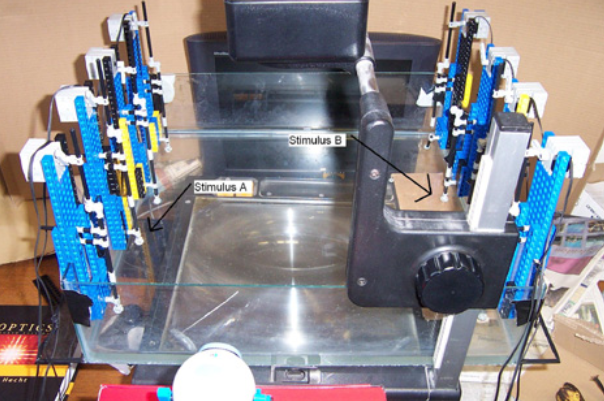
\includegraphics[width=\linewidth]{images/leterallyALiquidNetwork}
				\caption[A literal liquid network]{A literal liquid network. Source: \cite{10.1007/978-3-540-39432-7_63}}
				\label{fig:literallyaliquidnetwork}
			\end{figure}
	\end{columns}
\end{frame}
\begin{frame}
	\frametitle{Characteristics}
	\begin{itemize}
		\item \textbf{Adaptability}: Their dynamic nature enables them to respond dynamically to varying data distributions, making them well-suited for tasks involving non-stationary data.
		\item \textbf{Robustness}: LNNs have shown improved robustness against noise and input variations. The fluid-like behavior allows them to self-adjust and filter out irrelevant information, leading to enhanced generalization capabilities.
		\item \textbf{Exploration of Solution Space}: LNNs encourage solution space exploration by providing flexibility in the network's structure. The dynamic connectivity patterns enable the network to explore diverse pathways, potentially discovering novel solutions to complex problems.
		\item \textbf{Reduced Overfitting}: Due to their continuous learning capabilities, LNNs are less prone to overfitting, which often occurs in static networks, resulting in more accurate and generalizable models.
	\end{itemize}
\end{frame}
\begin{frame}
	\frametitle{Theory}
	\par To describe a LNN, we can use the equation \ref{eq:liquidRNN} \cite{Hasani2022} where at a time step t, $x(t)^{Dx1}$ defines the hidden state of a layer with D cells, and $I(t)^{Mx1}$ is the input to the system with $M$ features, $w_{\tau}^{Dx1}$ is a time-constant parameter vector,$A^{Dx1}$ is a bias vector, f is a neural network parametrized by $\theta$ and $\odot$ is the Hadamard product. The dependence of f(.) on x(t) denotes the possibility of having recurrent connections.
	
	\begin{equation}
		\label{eq:liquidRNN}
		\frac{d\mathbf{x}}{dt} = -[w_{\tau}^{Dx1} + f(\mathbf{x^{Dx1}}, \mathbf{I^{Mx1}}, \theta)] \odot \mathbf{x^{Dx1}}(t) + A^{Dx1} \odot f(\mathbf{x^{D^x1}}, \mathbf{I^{Mx1}}, \theta)
	\end{equation}


\end{frame}

\begin{frame}[allowframebreaks]
	\frametitle{Code}
	\par To illustrate, a simplified neuron is show below at the listing \ref{lst:liquidNeuron}:
	\input{listings/LiquidTimeConstantNeuron.py}
	\begin{figure}
		\centering
		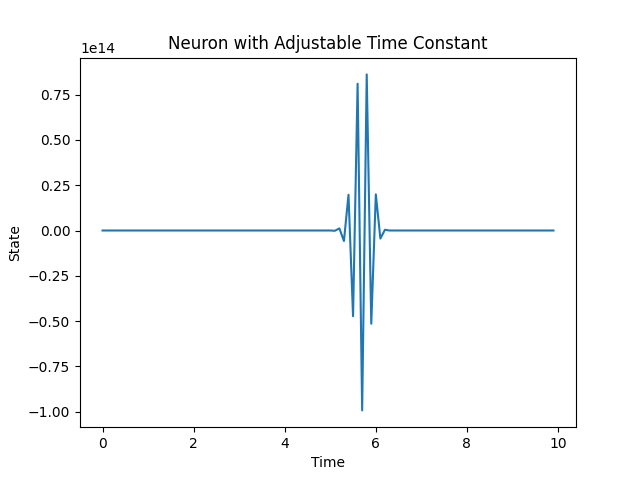
\includegraphics[width=0.35\linewidth]{images/liquidNeuron}
		\caption[A liquid neuron]{The liquid neuron of the listing \ref{lst:liquidNeuron} reacting to a continuous sinusoidal signal}
		\label{fig:liquidneuron}
	\end{figure}
	
	\par Then finally a pyTorch implementation \cite{liquid_nn_article}:
	\input{listings/LiquidNetwork.py}
\end{frame}
